%%%%%%%%%%%%%%%%%%%%%%%%%%%%%%%%%%%%%%%%%%%%%%%%%%%%%%%%%%%%%%%%%%%%%%%%%%%%%%%%

\documentclass[12pt, a4paper, oneside]{book}

\input{/home/giatro/.config/user/giatro_packages.tex}

\input{/home/giatro/.config/user/giatro_macros.tex}

\title{Deep Learning\\\small{by DeepLearning.AI}}
\date{\today}
\author{Lucas Paiolla Forastiere}

%%%%%%%%%%%%%%%%%%%%%%%%%%%%%%%%%%%%%%%%%%%%%%%%%%%%%%%%%%%%%%%%%%%%%%%%%%%%%%%%
%%%%%%%%%%%%%%%%%%%%%%%%%%%%%%%%%%%%%%%%%%%%%%%%%%%%%%%%%%%%%%%%%%%%%%%%%%%%%%%%

\begin{document}

\maketitle
\tableofcontents
\newpage

%%%%%%%%%%%%%%%%%%%%%%%%%%%%%%%%%%%%%%%%%%%%%%%%%%%%%%%%%%%%%%%%%%%%%%%%%%%%%

\chapter{Introduction}%
\label{cha:introduction}

The term deep learning refers to training \textit{neural networks}, sometimes
very big neural networks. But what are neural networks?

So let's suppose we want to predict housing prices based on the size of the
house. And let's say we'll use Logistic Regression to do that. But as we know,
house prices can't be negative, so we simply say the value of the house is $0$
if the Logistic Regression would predict something negative.

That's indeed the simplest neural network we can have, we have a single input
\texttt{size} and a single output \texttt{price} and in the middle we have a
single neuron: the logistic regression.

\begin{figure}[h]
\centering
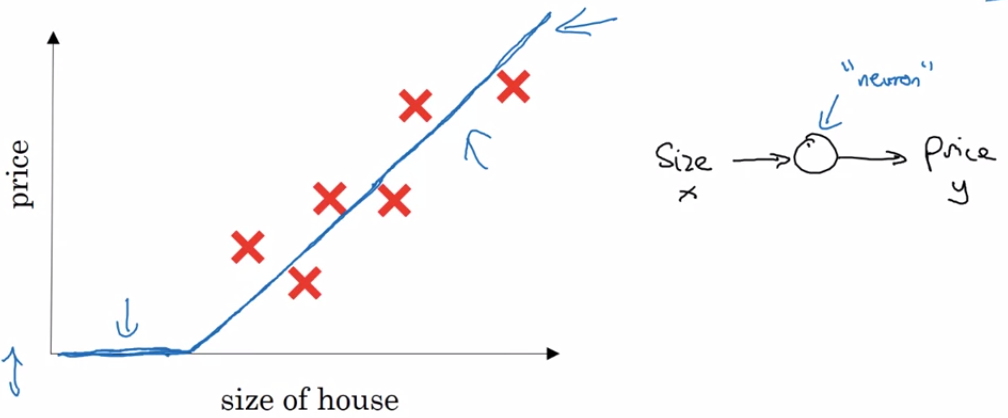
\includegraphics[scale=0.6]{Res/housing_logistic_regression.png}
\caption{Here we see the graph of the problem we described.}
\label{housing_logistic_regression.png}
\end{figure}

That function which is zero and than linear is called \textit{ReLU} and it's
used a lot in neural networks. It stands for \textit{Rectified Linear Unit}.

So to get a bigger neural network, we stack these neurons. Instead of predicting
using only the size of house, we could use the number of bedrooms, zip code and
wealth. We could use the size and number of bedrooms to predict the family size;
use the zip code to predict the walkability; and use the zip code and wealth to
predict the school quality. And then, we could use the family size, walkability
and school quality to predict the price. See in the picture:

\begin{figure}[h]
\centering
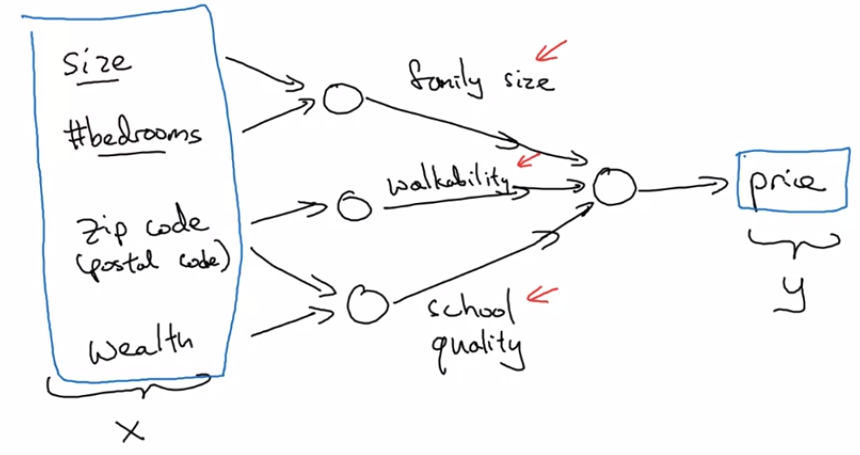
\includegraphics[scale=0.6]{Res/housing_nn.png}
\caption{Now we have a more complex neural network, which is the stack of many
ReLUs.}
\label{/housing_nn.png}
\end{figure}

However, in general what we have is something a little more complex than that.
We would have something like figure \ref{nn_generic.png}. Here we see that the
internal nodes (which are called \textbf{hidden nodes} or \textbf{hidden
neurons} or \textbf{hidden units}) receive the output of all the previous nodes
to make it predictions. These hidden nodes don't really have a meaning like the
example we gave. We don't try to predict family size or walkability or whatever,
we simply let the neural network decide what that neuron will output in order to
predict the final output \texttt{price} in the better way it can.

\begin{figure}[h]
\centering
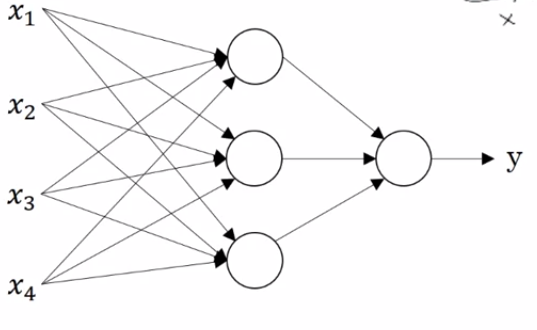
\includegraphics[scale=0.8]{Res/nn_generic.png}
\caption{The generic form of a neural network.}
\label{nn_generic.png}
\end{figure}

We can use neural networks in many applications, here we're going to foucos in
\textbf{supervised learning}, which are problems that you have a set of
variables called input (represented by $x$) and an output ($y$) related to that
input. In order to solve these kind of problems, there are many kinds of neural
networks. The one we saw is the most common one, but there are others, like
convolutional nn or recurrent nn.

\begin{figure}[h]
\centering
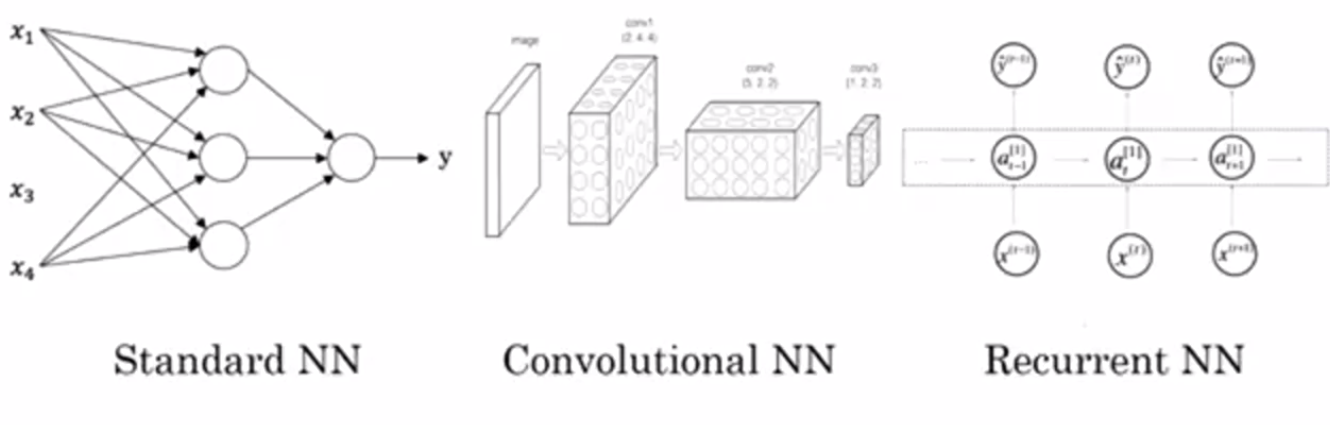
\includegraphics[scale=0.3]{Res/examples_nn.png}
\caption{Examples of neural networks.}
\label{examples_nn.png}
\end{figure}

Another thing that's important to decide what kind of nn we'll use is knowing if
the data we're leading with is \textit{structured} or \textit{unstructured}.

\textbf{Structured data} is data in the form of a table. We have a very clear
set of input variable $X$ and a set of output variables $y$. Each line of our
table represents one instance of data with many inputs and one or more outputs
related to those inputs.

\textbf{Unstructured data} is all the other kinds of data: audio, video, texts,
images, etc.

\begin{figure}[h]
\centering
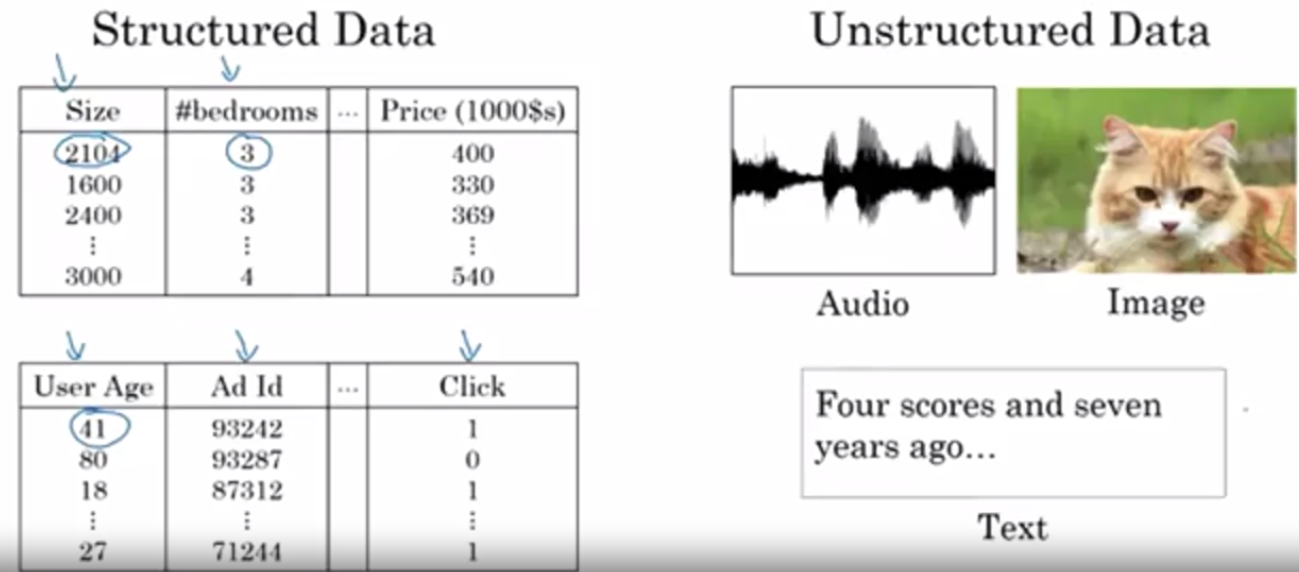
\includegraphics[scale=0.4]{Res/structured_vs_unstructed_data.png}
\caption{The two kinds of data.}
\label{structured_vs_unstructed_data.png}
\end{figure}

It turns out that machine learning algorithms performed better on structured
data over the years and more recently neural networks are performing better also
on unstructured data.

\paragraph{Why is Deep Learning taking off?}%
\label{par:why_is_deep_learning_taking_off_}

This is one of the questions we must ask ourselves when begining to learn deep
learning. Let's see the graph of the performance of the machine learning
algorithms versus the amount of data that we provide to then. We see that
traditional learning algorithms have a plato where they can't improve anymore,
which neural networks can lead with that data as we make than bigger and bigger.

\begin{figure}[h]
\centering
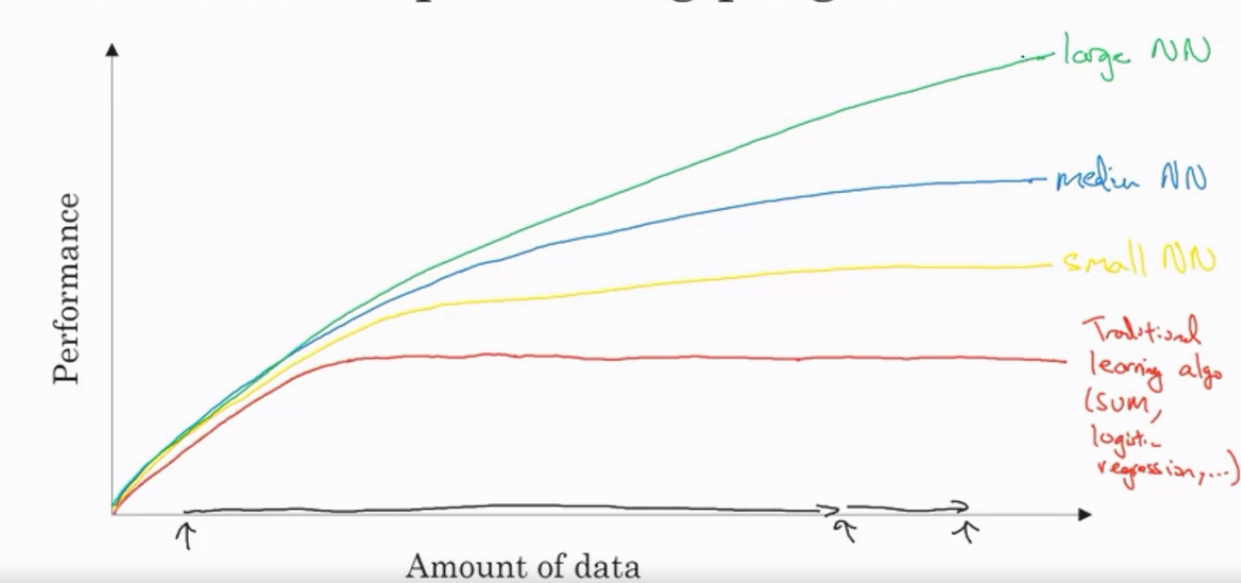
\includegraphics[scale=0.4]{Res/ml_algorithms_performance.png}
\caption{The performance of machine learning algorithms in respect to the data
we provide to them.}
\label{ml_algorithms_performance.png}
\end{figure}

We also see in the graph that when we don't have a large amount of data, NNs
all algorithms perform pretty much the same.

So in order to answer our question, we have to understand the evolution of three
things: \textit{data}, \textit{computation} and \textit{algorithms}.

Through the years, the amount of data available was inscreased a lot, so NNs can
take advantage from that. Also the computation power was inscreased with the use
of GPUs to make a large amount of computations. And finally new algorithms have
been developed to make NNs faster. That's the main reason why deep learning is
taking off.




%%%%%%%%%%%%%%%%%%%%%%%%%%%%%%%%%%%%%%%%%%%%%%%%%%%%%%%%%%%%%%%%%%%%%%%%%%%%%%%%

\end{document}
